\chapter{Background and Related Work}\label{ch:background}

\section{Introduction}\label{sec:bg-intro}
The two controllers of this thesis act on the settings that connect a detector and a tracker. To follow their design and evaluation, the reader needs to know how a detector produces its boxes and scores, how a tracker turns these boxes into tracks, how the scores enter the tracker's decisions, what makes aerial video difficult, and how tracking accuracy is measured. Section~\ref{sec:bg-technical} provides this background. Section~\ref{sec:bg-detection} introduces object detection and the three settings of the detector operating point, and Section~\ref{sec:bg-detectors} reviews deep learning-based detectors, including those used in this thesis. Section~\ref{sec:bg-mot} defines multi-object tracking and its constraints, Section~\ref{sec:bg-paradigms} describes the tracking paradigms, and Section~\ref{sec:bg-association} reviews data association and track management in the trackers used in this work. Section~\ref{sec:bg-confidence} explains how trackers use detector scores, why these scores differ between detectors, and the thresholding tools on which SCL builds. Section~\ref{sec:bg-datasets} describes the difficulties of aerial tracking and the datasets of the thesis, and Section~\ref{sec:bg-metrics} defines the evaluation metrics and the experimental protocol shared by Chapters~\ref{ch:acmot} and~\ref{ch:scl}. Sections~\ref{sec:bg-detection}--\ref{sec:bg-datasets} extend the survey published by the author \cite{ismail2026realtime}. Section~\ref{sec:rw} then reviews the related work by theme, compares the closest methods with the proposed controllers, and states the research gap, and Section~\ref{sec:bg-summary} summarizes the chapter.

\section{Technical Background}\label{sec:bg-technical}

\subsection{Object Detection Fundamentals}\label{sec:bg-detection}
Object detection and tracking have evolved through three technological phases \cite{li2025motreview,ismail2026realtime}. Before 2012, detectors relied on hand-engineered features such as the histogram of oriented gradients \cite{dalal2005hog} and scale-invariant keypoints \cite{lowe2004sift}, combined with sliding windows and shallow classifiers. The second phase began when CNNs trained on large labeled datasets \cite{krizhevsky2017alexnet,russakovsky2015imagenet} outperformed hand-crafted features; region-based detectors \cite{girshick2014rcnn,ren2017fasterrcnn} and single-stage detectors \cite{redmon2016yolo,liu2016ssd} pushed the accuracy--speed frontier, and deep residual networks \cite{he2016resnet} became standard backbones. The third phase, beginning around 2020, introduced attention-based models \cite{vaswani2017attention,dosovitskiy2021vit}: the detection transformer (DETR) \cite{carion2020detr} removed hand-designed anchors and NMS, and transformer-based trackers integrated detection and association in one network \cite{sun2020transtrack,meinhardt2022trackformer,zeng2022motr}.

Whatever its architecture, a detector maps an image $I_t$ to a set of candidates
\begin{equation}
\mathcal{D}_t = \{(\mathbf{x}_{t,i}, s_{t,i}, c_{t,i})\}_{i=1}^{n_t},
\label{eq:bg-dets}
\end{equation}
where $\mathbf{x}_{t,i}$ is a bounding box, $s_{t,i}\in(0,1)$ a confidence score, and $c_{t,i}$ a class label \cite{ismail2026realtime}. The overlap of two boxes $A$ and $B$ is measured by their intersection over union (IoU),
\begin{equation}
\mathrm{IoU}(A,B)=\frac{|A\cap B|}{|A\cup B|},
\label{eq:bg-iou}
\end{equation}
the area of their intersection divided by the area of their union, which is 1 for identical boxes and 0 for disjoint ones.

Three settings, chosen by the user when the detector is run, decide which candidates leave the detector. The \emph{confidence threshold} removes every candidate whose score is below it; a higher threshold passes fewer but more reliable boxes. \emph{Non-maximum suppression} (NMS) removes duplicates: candidates are visited in order of decreasing score, and a candidate is removed when its IoU with a higher-scoring kept candidate exceeds the NMS IoU threshold, so a lower threshold removes more overlapping boxes. The \emph{input resolution} is the size to which every frame is resized before inference; a larger input shows small objects better but increases the computation. Together, these three values form the detector operating point, the variable that AC-MOT controls in Chapter~\ref{ch:acmot}.

Detection quality is commonly reported with the average precision (AP), the area under the precision--recall curve of one class at one IoU threshold, and its mean over classes and thresholds (mAP), together with the speed in frames per second (FPS) \cite{lin2014coco,ismail2026realtime}. These detection metrics judge every frame on its own; the tracking metrics used in this thesis are introduced in Section~\ref{sec:bg-metrics}.

\subsection{Deep Learning-Based Object Detectors}\label{sec:bg-detectors}
Object detectors are broadly divided into two-stage and single-stage architectures, with transformer-based detectors forming a third group \cite{ismail2026realtime}. Table~\ref{tab:bg-detectors} summarizes the detectors discussed in this section.

\emph{Two-stage detectors.} The region-based CNN (R-CNN) family first proposes candidate regions and then classifies and refines them \cite{girshick2014rcnn}. Faster R-CNN introduced a region proposal network that shares convolutional features with the detection head, which made the proposals nearly free and improved both speed and accuracy \cite{ren2017fasterrcnn}. Mask R-CNN added a parallel branch that predicts a segmentation mask for each detection \cite{he2017maskrcnn}. Two-stage detectors are accurate, particularly for small objects and cluttered scenes, but they are generally slower than single-stage detectors.

\emph{Single-stage detectors.} Single-stage detectors predict boxes and class probabilities in one pass over the image. The YOLO (You Only Look Once) family treats detection as a regression problem over a grid \cite{redmon2016yolo}; successive versions improved the backbone, the neck, and the training recipe \cite{redmon2018yolov3,bochkovskiy2020yolov4,ge2021yolox,wang2024yolov9}, and recent generations distributed as software libraries, such as YOLOv8 \cite{jocher2023yolov8} and YOLO11 \cite{jocher2024yolo11}, offer a range of model sizes. The Single Shot MultiBox Detector (SSD) predicts boxes from feature maps at several scales \cite{liu2016ssd}. RetinaNet introduced the focal loss to address the imbalance between foreground and background during the training of dense detectors \cite{lin2017focal}. EfficientDet combined a bidirectional feature pyramid with compound scaling of resolution, depth, and width \cite{tan2020efficientdet}. Feature pyramid networks \cite{lin2017fpn} are a common architectural response to scale variation.

\emph{Transformer-based detectors.} DETR formulates detection as set prediction with a transformer encoder--decoder, which removes anchors and NMS \cite{carion2020detr}. The original DETR converges slowly and is expensive. Real-time transformer detectors such as RT-DETR \cite{zhao2024rtdetr} and RF-DETR \cite{robinson2025rfdetr} keep the set-prediction formulation while reducing latency to the range of single-stage detectors.

\begin{table}[tbp]
\centering
\caption{Detector families discussed in this thesis. The last column gives the thresholds that the user chooses when the detector is run.}
\label{tab:bg-detectors}
\begin{tabular}{>{\raggedright\arraybackslash}p{2.9cm}>{\raggedright\arraybackslash}p{1.0cm}>{\raggedright\arraybackslash}p{2.4cm}>{\raggedright\arraybackslash}p{4.1cm}>{\raggedright\arraybackslash}p{2.4cm}}
\toprule
Detector & Year & Architecture & Key idea & User thresholds \\
\midrule
R-CNN \cite{girshick2014rcnn} & 2014 & two-stage & CNN features on region proposals & confidence, NMS \\
Faster R-CNN \cite{ren2017fasterrcnn} & 2017 & two-stage & shared region proposal network & confidence, NMS \\
Mask R-CNN \cite{he2017maskrcnn} & 2017 & two-stage & parallel mask branch & confidence, NMS \\
YOLO \cite{redmon2016yolo} & 2016 & single-stage & grid regression of boxes and classes & confidence, NMS \\
SSD \cite{liu2016ssd} & 2016 & single-stage & multi-scale default boxes & confidence, NMS \\
RetinaNet \cite{lin2017focal} & 2017 & single-stage & focal loss for class imbalance & confidence, NMS \\
EfficientDet \cite{tan2020efficientdet} & 2020 & single-stage & bidirectional pyramid, compound scaling & confidence, NMS \\
YOLOX \cite{ge2021yolox} & 2021 & single-stage & anchor-free, decoupled head & confidence, NMS \\
DETR \cite{carion2020detr} & 2020 & transformer & set prediction, no NMS & confidence \\
RT-DETR \cite{zhao2024rtdetr} & 2024 & transformer & real-time hybrid encoder & confidence \\
\bottomrule
\end{tabular}
\end{table}

\emph{Detectors used in this thesis.} AC-MOT controls the YOLO11m detector \cite{jocher2024yolo11} of the Ultralytics YOLO family, in a public version trained on VisDrone2019-DET \cite{zhu2022visdrone}. SCL is evaluated on four detection sources: the published YOLOX-X detections of the MOT17 benchmark \cite{ge2021yolox}, the detections released by the authors of two external trackers, and two detectors that the trackers were not tuned for, YOLOv8n \cite{jocher2023yolov8} and RT-DETR-L \cite{zhao2024rtdetr}. The three families produce different score distributions, which is the situation that SCL addresses.

\subsection{Multi-Object Tracking Fundamentals}\label{sec:bg-mot}
Multi-object tracking associates detections across time into trajectories $\mathcal{T}=\{\tau_j\}$, each a sequence of boxes of one object between a start frame and an end frame \cite{ismail2026realtime}. An online tracker processes the video frame by frame and solves, in each frame, an assignment problem
\begin{equation}
\pi_t^{*} = \arg\min_{\pi_t} \sum_{(i,j)\in\pi_t} C\left(\mathbf{x}_{t,i}, \tau_j\right),
\label{eq:bg-assign}
\end{equation}
where $\pi_t$ is a one-to-one matching between the detections of frame $t$ and the existing tracks, and $C$ is a cost based on predicted motion, appearance, or learned embeddings. The Hungarian method \cite{kuhn1955hungarian} solves this assignment exactly, and a Kalman filter \cite{kalman1960} is the usual motion predictor. The quality of $\mathcal{T}$ therefore depends on the detections that enter Eq.~\eqref{eq:bg-assign} as much as on the cost and the assignment: missed detections break trajectories, and false detections cause wrong associations and identity switches.

\emph{Applications and challenges.} Real-time detection and tracking are required wherever a system must perceive its environment continuously. Surveillance and security systems track people and vehicles in live streams; driver assistance and autonomous driving rely on real-time detection of pedestrians, vehicles, and obstacles \cite{geiger2012kitti}; and UAVs apply detection and tracking in traffic monitoring, inspection, search, and defense \cite{zhu2022visdrone,bakirci2025lowpower}. The aerospace literature has studied airborne target tracking \cite{miller2015multitarget,desai2017uavfeature}, onboard deep detection \cite{lu2024uavdetection,choi2022docking}, and vision-based guidance \cite{parsons2019refueling}. Across these applications, MOT faces three coupled problems: detecting the objects, associating detections across frames, and keeping identities through occlusion \cite{li2025motreview,ismail2026realtime}.

\emph{Real-time constraints.} Real-time performance is limited by three factors \cite{bakirci2025lowpower,ismail2026realtime}. The first is the accuracy--speed trade-off: more accurate models generally need more computation and longer inference. The second is the hardware, which ranges from data-center graphics processing units (GPUs) to low-power embedded processors on board a vehicle or an aircraft. The third is the deployment context: bandwidth, power supply, and the need for onboard rather than remote processing. In a tracking pipeline these constraints act mainly through the detector, whose input resolution sets most of the cost, while the tracker itself is usually inexpensive. A controller that changes the detector's resolution therefore also changes the cost of the pipeline, and a controller placed between the detector and the tracker must itself be cheap.

\subsection{Tracking-by-Detection Architectures}\label{sec:bg-paradigms}
Three paradigms organize the MOT literature \cite{ismail2026realtime,adzemovic2026survey}.

\emph{Tracking by detection.} A detector is applied independently to every frame, and an online tracker associates the detections over time using motion and appearance cues \cite{bewley2016sort,wojke2017deepsort}. The paradigm benefits directly from advances in detectors and remains modular: any detector can feed any tracker. Its interface is the set of candidates of Eq.~\eqref{eq:bg-dets}, filtered first by the detector operating point and then by the tracker's score thresholds. It is the paradigm used throughout this thesis, because it is the one in which detectors and trackers are combined and exchanged independently, and therefore the one in which their settings must be reconciled.

\emph{Joint detection and tracking.} Joint detection and embedding (JDE) learns detection and appearance embeddings in a shared model \cite{wang2020jde}; FairMOT treats detection and re-identification (ReID) as equally important tasks with an anchor-free design \cite{zhang2021fairmot}; and CenterTrack predicts object centers and their displacements between frames \cite{zhou2020centertrack}. These methods reduce the cost of a separate appearance model, but they couple the detector and the tracker, so that neither can be exchanged independently.

\emph{Transformer-based tracking.} TransTrack propagates queries between frames \cite{sun2020transtrack}; TrackFormer separates object queries for new objects from track queries for existing ones \cite{meinhardt2022trackformer}; MOTR carries track queries across frames and updates them by attention \cite{zeng2022motr}; and MOTIP predicts identities directly \cite{gao2025motip}. These methods are fully differentiable, but they remain computationally expensive, and their thresholds are internal to the network.

\subsection{Data Association and Track Management}\label{sec:bg-association}
A tracking-by-detection tracker repeats three operations in every frame: it predicts where each existing track should be, associates the new detections with these predictions, and manages the life of the tracks. A track is \emph{born} from a detection that matches no track and whose score passes the birth threshold; it is \emph{continued} by matched detections; and it is \emph{lost} and finally removed when no detection has matched it for a number of frames, the track buffer. This section reviews the trackers used or discussed in the thesis, with attention to how each of them uses detector scores; Table~\ref{tab:bg-trackers} summarizes them.

\emph{Motion-based trackers.} Simple online and realtime tracking (SORT) combines a constant-velocity Kalman filter with Hungarian assignment on box overlap \cite{bewley2016sort}. It is simple and fast, but it relies on motion alone, so occlusion and irregular motion cause many identity switches. The IOU tracker shows how far pure overlap association can go at high frame rates \cite{bochinski2017iou}. ByteTrack introduced a second association step: detections above a high threshold are associated first, and the tracks that remain unmatched are then associated with low-confidence detections, which recovers partially occluded objects that other trackers discard \cite{zhang2022bytetrack}. OC-SORT refines the Kalman filter with an observation-centric re-update and a velocity-direction consistency term, which improves robustness to occlusion and non-linear motion \cite{cao2023ocsort}; it uses a single confidence threshold. Buffered IoU matching enlarges the boxes during association to handle irregular motion \cite{yang2023cbiou}.

\emph{Motion and appearance trackers.} DeepSORT adds deep appearance embeddings to SORT and combines the Kalman prediction with the cosine distance between embeddings, which reduces identity switches \cite{wojke2017deepsort}. BoT-SORT adds camera-motion compensation, an improved Kalman state, and ReID features to the ByteTrack association \cite{aharon2022botsort}. StrongSORT revisits DeepSORT with an exponential moving average of appearance features, camera-motion compensation by the enhanced correlation coefficient \cite{evangelidis2008ecc}, and other refinements \cite{du2023strongsort}. Deep OC-SORT adds adaptive appearance re-identification to OC-SORT \cite{maggiolino2023deepocsort}, and SMILEtrack learns similarity for occlusion-aware association \cite{wang2024smiletrack}.

\emph{Recent trackers used in this thesis.} Hybrid-SORT uses weak cues, such as the confidence state and the height of a box, alongside strong cues \cite{yang2024hybridsort}. SparseTrack decomposes crowded scenes by pseudo-depth before association \cite{liu2025sparsetrack}. BoostTrack boosts the confidence of likely true detections and augments the similarity measure \cite{stanojevic2024boosttrack}. PD-SORT adds pseudo-depth cues to the motion model to handle occlusion \cite{wang2025pdsort}. U2MOT is an uncertainty-aware tracker trained without identity labels \cite{liu2023u2mot}. OATrack \cite{qi2026oatrack} is a recent tracker for small objects in UAV video; it weights association by detection quality, uses a YOLO detection cache, and has a fixed tracker-side confidence gate.

\begin{table}[tbp]
\centering
\caption{Tracking-by-detection trackers discussed in this thesis and how they use detector scores. The last column names the chapter in which a tracker is used.}
\label{tab:bg-trackers}
\begin{tabular}{>{\raggedright\arraybackslash}p{2.5cm}>{\raggedright\arraybackslash}p{0.9cm}>{\raggedright\arraybackslash}p{4.1cm}>{\raggedright\arraybackslash}p{2.9cm}>{\raggedright\arraybackslash}p{2.4cm}}
\toprule
Tracker & Year & Main cues & Score use & Used with \\
\midrule
SORT \cite{bewley2016sort} & 2016 & Kalman motion, IoU & one threshold & background \\
DeepSORT \cite{wojke2017deepsort} & 2017 & motion, appearance & one threshold & background \\
ByteTrack \cite{zhang2022bytetrack} & 2022 & motion, IoU, low-score recovery & two stages & AC-MOT, SCL \\
BoT-SORT \cite{aharon2022botsort} & 2022 & motion, camera motion, ReID & two stages & SCL \\
OC-SORT \cite{cao2023ocsort} & 2023 & observation-centric motion & one threshold & SCL \\
StrongSORT \cite{du2023strongsort} & 2023 & motion, appearance, camera motion & one threshold & background \\
U2MOT \cite{liu2023u2mot} & 2023 & uncertainty-aware association & published static setting & AC-MOT development \\
Hybrid-SORT \cite{yang2024hybridsort} & 2024 & strong and weak cues & two stages & SCL \\
BoostTrack \cite{stanojevic2024boosttrack} & 2024 & confidence boost, similarity & two stages & SCL \\
SparseTrack \cite{liu2025sparsetrack} & 2025 & pseudo-depth decomposition & two stages & AC-MOT development, SCL \\
PD-SORT \cite{wang2025pdsort} & 2025 & pseudo-depth motion & one threshold & SCL \\
OATrack \cite{qi2026oatrack} & 2026 & quality-weighted association & confidence gate & AC-MOT \\
\bottomrule
\end{tabular}
\end{table}

\subsection{Detector Confidence Scores and Thresholding}\label{sec:bg-confidence}
\emph{How trackers use detector scores.} All of the trackers above read detector scores through fixed thresholds that their authors tuned for one detector, usually YOLOX \cite{ge2021yolox} on MOT17. Two kinds of trackers can be distinguished (Fig.~\ref{fig:bg-stages}). A \emph{single-stage} tracker, such as OC-SORT, ignores every box below one threshold. A \emph{two-stage} tracker, such as ByteTrack, uses boxes above a high threshold to match tracks and boxes above a higher threshold to start tracks, and it uses lower-score boxes, down to a low threshold, in a second step that can only continue tracks left unmatched by the first step. If a detector gives scores on a different scale from the one for which the thresholds were tuned, a single-stage tracker can lose most of its boxes, and a two-stage tracker can lose its ability to start tracks. Published comparisons show the steady progress of tracking accuracy from motion-only methods to trackers that combine motion, appearance, and low-score association \cite{ismail2026realtime}; they compare trackers on one fixed set of detections, however, and do not show how a tracker behaves when its detector changes.

\begin{figure}[tbp]
\centering
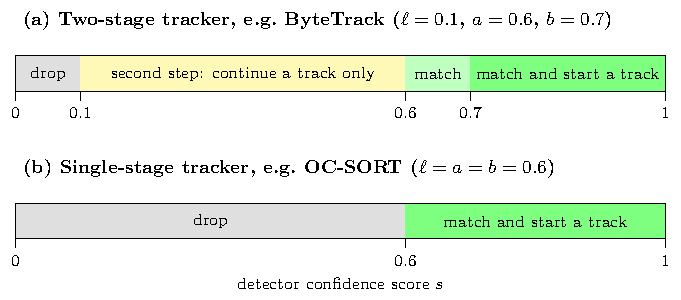
\includegraphics[width=0.9\textwidth]{figures/score_stages.pdf}
\caption{How a two-stage and a single-stage tracker use the detector score, with the published thresholds of ByteTrack (official setting) and OC-SORT. $\ell$: lowest score used; $a$: score needed to match a track; $b$: score needed to start a track.}
\label{fig:bg-stages}
\end{figure}

\emph{Confidence and calibration.} A classifier is calibrated when its confidence equals its probability of being correct. Modern neural networks are often poorly calibrated \cite{guo2017calibration}, and object detectors are no exception: their confidence depends on the position and size of the box as well as on the class, and it shifts with the data \cite{kuppers2020detcalib}. Detectors of different families \cite{redmon2016yolo,ren2017fasterrcnn,carion2020detr,zhao2024rtdetr,wang2024yolov9} produce different score distributions, and soft suppression changes the scores of overlapping boxes \cite{bodla2017softnms}. The same object may therefore receive 0.9 from one detector and a much lower score from another. Calibration methods fit a mapping from scores to probabilities on labeled data \cite{kuppers2020detcalib}, which is not possible when a detector is exchanged in a deployed pipeline without labels. Test-time adaptation methods adapt a model to unlabeled data \cite{wang2021tent}, but they change the model's weights, whereas this thesis keeps both the detector and the tracker frozen.

\emph{Logits.} A score $s\in(0,1)$ can be written as its logit, the log-odds
\begin{equation}
z=\log\frac{s}{1-s},
\label{eq:bg-logit}
\end{equation}
which keeps the order of the scores and spreads out the regions near 0 and 1 where detector scores crowd; the logistic function $\sigma(z)=1/(1+e^{-z})$ maps a logit back to a score. A common change of a detector's scores, a change of temperature, divides all logits by the same number.

\emph{Label-free thresholding.} Classical image thresholding offers a tool that needs no labels. Otsu's method chooses the threshold that best splits a histogram into two groups \cite{goh2018otsu}. For a candidate threshold $k$, let $\omega_0(k)$ and $\omega_1(k)$ be the fractions of values below and above $k$, and $\mu_0(k)$ and $\mu_1(k)$ their means. The method selects
\begin{equation}
k^{*}=\arg\max_{k}\;\omega_0(k)\,\omega_1(k)\,\bigl(\mu_0(k)-\mu_1(k)\bigr)^2,
\label{eq:bg-otsu}
\end{equation}
the threshold that maximizes the between-class variance. It adapts to the shape of the distribution, and it moves with any stretch or shift of the values. SCL applies it to the logits of recent detector scores (Chapter~\ref{ch:scl}).

\subsection{Aerial Tracking Challenges and Datasets}\label{sec:bg-datasets}
\emph{Difficulties of aerial video.} Aerial video adds small targets, changing object counts, camera motion, and clutter to the general difficulties of MOT \cite{zhu2022visdrone,du2018uavdt}. Small objects produce few pixels and low detector confidence \cite{cheng2023smallobject}; the number of objects changes quickly in traffic; the moving camera changes position, altitude, and viewing angle; and illumination, background, and occlusion vary within one video. These properties make the detector operating point especially important: a larger input helps small objects, while the confidence and NMS thresholds change how many detections reach the tracker.

\emph{Datasets of the field.} Detection models are commonly trained on COCO (Common Objects in Context), which contains more than 330,000 images with annotations for 80 object categories \cite{lin2014coco}, and ImageNet provides the large-scale classification data on which most backbones are pretrained \cite{russakovsky2015imagenet}. For tracking, the MOTChallenge benchmarks MOT16 and MOT17 \cite{milan2016mot16,dendorfer2021motchallenge} contain pedestrian sequences from static and moving cameras, and MOT20 contains very crowded scenes \cite{dendorfer2020mot20}. DanceTrack contains dancers with uniform appearance and diverse motion, which makes association by appearance difficult \cite{sun2022dancetrack}. The four datasets used in this thesis are described below, and Table~\ref{tab:bg-data} lists the splits and the role of each one.

\emph{VisDrone2019-MOT.} VisDrone2019-MOT is a widely used benchmark for MOT in UAV videos \cite{zhu2022visdrone}. It contains video sequences recorded by various drone-mounted cameras in 14 cities in China, in urban and rural regions and in both sparse and crowded scenes. The VisDrone benchmark annotates ten object categories, such as pedestrians, cars, buses, and bicycles, with boxes that give the location and identity of each tracked object. Its MOT track uses 96 video clips: 56 for training (24,198 frames), 7 for validation (2,846 frames), 16 for challenge testing (6,322 frames), and 17 for development testing (6,635 frames). Although ten categories are annotated, the official MOT evaluation scores only five of them: pedestrian, car, van, bus, and truck \cite{zhu2022visdrone}.

\emph{UAVDT.} UAVDT is a benchmark designed for object detection and MOT in UAV videos, with a particular focus on vehicles \cite{du2018uavdt}. It consists of 100 video sequences selected from more than 10 hours of video recorded at urban locations such as squares, arterial streets, toll stations, highways, crossings, and T-junctions, at 30 frames per second and a resolution of $1080\times540$ pixels. About 80,000 frames are annotated with 0.84 million boxes of vehicles in three categories: car, truck, and bus. The sequences are recorded under different weather conditions, flying altitudes, and camera viewing angles, which change object size, visibility, and the number of vehicles per frame. The test set contains 20 sequences for the MOT task (16,592 frames) \cite{du2018uavdt}.

\emph{MOT17.} MOT17 \cite{milan2016mot16} contains 14 sequences of people filmed with static and moving cameras. As is common, the second half of each of the seven training sequences, called val-half (2,652 frames), is used for evaluation \cite{zhang2022bytetrack}. The benchmark distributes detections of a published YOLOX-X detector \cite{ge2021yolox} that are used by many trackers.

\emph{KITTI tracking.} KITTI tracking \cite{geiger2012kitti} has 21 training sequences (8,008 frames) recorded from a car and is scored on cars and pedestrians.

\begin{table}[tbp]
\centering
\caption{Datasets and splits used in this thesis and the role of each one.}
\label{tab:bg-data}
\begin{tabular}{>{\raggedright\arraybackslash}p{2.8cm}>{\raggedright\arraybackslash}p{4.4cm}>{\raggedright\arraybackslash}p{1.9cm}>{\raggedright\arraybackslash}p{4.3cm}}
\toprule
Dataset & Split & Controller & Role\\
\midrule
VisDrone2019-MOT & training, 8 sequences (3,282 frames) & AC-MOT & calibration (tuning) data\\
VisDrone2019-MOT & validation, 7 sequences (2,846 frames) & AC-MOT & frozen evaluation\\
UAVDT & test, 20 sequences (16,592 frames) & AC-MOT & transfer without retuning\\
MOT17 & val-half, 7 sequences (2,652 frames) & SCL & development; predeclared external trackers\\
KITTI tracking & training, 21 sequences (8,008 frames) & SCL & development under a detector change\\
UAVDT & test, 20 sequences (16,592 frames) & SCL & held-out evaluation, run once\\
\bottomrule
\end{tabular}
\end{table}

\subsection{Evaluation Metrics and Experimental Protocols}\label{sec:bg-metrics}
Eight commonly used MOT metrics are considered: HOTA, MOTA, IDF1, IDS, false positives (FP), false negatives (FN), precision, and recall. They measure different aspects of tracking performance, including detection accuracy, the consistency of object identities, and the ability to follow objects across consecutive frames \cite{dendorfer2021motchallenge,luiten2021hota}. They are defined below, starting from the errors counted in each frame and ending with the scores that combine them.

\emph{Detection errors.} In each frame $t$, output boxes are matched one to one to ground-truth boxes with an IoU of at least 0.5. Let $\mathrm{GT}_t$ be the number of ground-truth boxes, $\mathrm{TP}_t$ the number of matched pairs (true positives), $\mathrm{FP}_t$ the number of output boxes without a match, and $\mathrm{FN}_t$ the number of ground-truth boxes without a match (missed objects). Over all frames,
\begin{align}
\mathrm{GT}&=\sum_t \mathrm{GT}_t,\qquad \mathrm{TP}=\sum_t \mathrm{TP}_t,\label{eq:bg-gt}\\
\mathrm{FP}&=\sum_t \mathrm{FP}_t,\qquad \mathrm{FN}=\sum_t \mathrm{FN}_t,\label{eq:bg-fpfn}
\end{align}
so that $\mathrm{TP}=\mathrm{GT}-\mathrm{FN}$. Precision is the fraction of output boxes that are correct, and recall is the fraction of ground-truth boxes that are found:
\begin{equation}
\mathrm{Precision}=\frac{\mathrm{TP}}{\mathrm{TP}+\mathrm{FP}},\qquad
\mathrm{Recall}=\frac{\mathrm{TP}}{\mathrm{GT}}.
\label{eq:bg-prrc}
\end{equation}

\emph{Identity switches.} The counts above treat each frame separately, so they do not show whether an object keeps the same track over time. Let $\phi_t(i)$ be the output track matched to ground-truth object $i$ in frame $t$, and $\phi_{\mathrm{prev}}(i)$ the output track to which object $i$ was last matched before $t$. An identity switch is counted whenever these two tracks differ:
\begin{equation}
\mathrm{IDS}=\sum_t\sum_{i}\mathbf{1}\!\left[\phi_t(i)\neq\phi_{\mathrm{prev}}(i)\right],
\label{eq:bg-ids}
\end{equation}
where the inner sum runs over the objects that are matched in frame $t$ and were matched before, and the indicator $\mathbf{1}[\cdot]$ is 1 when its condition holds and 0 otherwise.

\emph{MOTA and IDF1.} These two scores summarize the errors above in one number each \cite{bernardin2008clear,ristani2016idf1}. MOTA combines the three error types, and IDF1 measures how long each object keeps the correct identity:
\begin{align}
\mathrm{MOTA}&=1-\frac{\mathrm{FN}+\mathrm{FP}+\mathrm{IDS}}{\mathrm{GT}},\label{eq:bg-mota}\\
\mathrm{IDF1}&=\frac{2\,\mathrm{IDTP}}{2\,\mathrm{IDTP}+\mathrm{IDFP}+\mathrm{IDFN}}.\label{eq:bg-idf1}
\end{align}
For IDF1, each ground-truth track is first matched to at most one output track over the whole video; IDTP, IDFP, and IDFN are then the true-positive, false-positive, and false-negative boxes under this track-level matching. Because MOTA counts every false positive and every missed object, it reacts strongly to how many boxes the detector passes on, and it becomes negative when the errors outnumber the ground-truth boxes. IDF1 depends more on whether each object keeps one identity.

\emph{HOTA.} MOTA depends mostly on detection errors, and IDF1 mostly on identity errors. HOTA balances detection and association in one score \cite{luiten2021hota}. At a localization threshold $\alpha$, let $\mathrm{TP}_\alpha$, $\mathrm{FN}_\alpha$, and $\mathrm{FP}_\alpha$ be the matched pairs, missed ground-truth boxes, and unmatched output boxes. For a matched pair $c$, $\mathrm{TPA}(c)$ is the set of matched pairs with the same ground-truth identity and the same output identity as $c$; $\mathrm{FNA}(c)$ is the set of boxes of the same ground-truth object that are matched to another output identity or not matched; and $\mathrm{FPA}(c)$ is the set of boxes of the same output track that are matched to another object or not matched. Then
\begin{align}
\mathrm{DetA}_\alpha&=\frac{|\mathrm{TP}_\alpha|}{|\mathrm{TP}_\alpha|+|\mathrm{FN}_\alpha|+|\mathrm{FP}_\alpha|},\label{eq:bg-deta}\\
\mathcal{A}(c)&=\frac{|\mathrm{TPA}(c)|}{|\mathrm{TPA}(c)|+|\mathrm{FNA}(c)|+|\mathrm{FPA}(c)|},\label{eq:bg-ac}\\
\mathrm{AssA}_\alpha&=\frac{1}{|\mathrm{TP}_\alpha|}\sum_{c\in\mathrm{TP}_\alpha}\mathcal{A}(c),\label{eq:bg-assa}\\
\mathrm{HOTA}&=\frac{1}{19}\sum_{\alpha}\sqrt{\mathrm{DetA}_\alpha\,\mathrm{AssA}_\alpha},\label{eq:bg-hota}
\end{align}
where $\alpha$ runs over $0.05, 0.10, \dots, 0.95$; $\mathrm{DetA}$ is the detection accuracy and $\mathrm{AssA}$ the association accuracy.

\emph{Units and direction.} HOTA, MOTA, IDF1, precision, and recall are given in percent, and differences in points; IDS, FP, and FN are counts; speed is given in FPS, and runtime in milliseconds (ms) per frame. Higher values are better for HOTA, MOTA, IDF1, precision, recall, and FPS, and lower values are better for IDS, FP, FN, and runtime.

\emph{Paired comparison and bootstrap intervals.} Every comparison in this thesis is paired: the same tracker runs with fixed settings and with a controller on the same sequences and detections, and nothing else changes. To judge whether the difference between two systems is reliable, paired bootstrap resampling is applied at the sequence level \cite{efron2016casi}, which keeps the dependence within each sequence. Each resample draws the evaluation sequences with replacement; the same draw is used for both systems, the pooled metrics are recomputed, and their difference is recorded. The 95\% confidence interval (CI) is the 2.5--97.5 percentile range, and a difference is called reliable (significant) when its interval does not include zero. Because whole sequences are resampled, the intervals reflect the variation between videos, not only between frames. The number of resamples is given in each chapter.

\emph{Development, calibration, and evaluation data.} Both controllers follow the same protocol. Their values are chosen only on development or calibration data, the configuration is then frozen, and only the frozen configuration is run on the evaluation data. The UAVDT test split, used by both controllers, and the predeclared external trackers of SCL were run once with the frozen configuration. Detector and tracker parameters affect accuracy, identity consistency, and speed in conflicting ways, so the development of AC-MOT used systematic search with Optuna and its tree-structured Parzen estimator (TPE) sampler \cite{akiba2019optuna}, on calibration data only.

\section{Related Work}\label{sec:rw}
This section reviews the work closest to the two controllers, organized by theme rather than by publication: the tracking-by-detection systems that the controllers serve, methods that adapt the detector, methods that adapt the thresholds of a tracker, and methods that calibrate scores or connect different trackers to a detector. It ends with a comparison of the closest methods and the research gap that this thesis addresses.

\subsection{Tracking-by-Detection Systems and Aerial MOT}\label{sec:rw-tbd}
In tracking by detection, objects are detected in each frame and associated across frames, and most methods improve motion prediction or association for a given detector. SORT built a compact online pipeline from motion prediction and assignment \cite{bewley2016sort}; StrongSORT adds appearance features to reduce identity fragmentation \cite{du2023strongsort}; ByteTrack associates high-confidence detections first and then uses low-confidence boxes to recover objects that would otherwise be lost \cite{zhang2022bytetrack}; and OC-SORT uses one score threshold with an observation-centric motion model \cite{cao2023ocsort}. Many recent trackers improve association further with trained or domain-specific parts \cite{li2024fdbtrack,bao2024graphmatching,zhang2025sinkhorn,ding2025remot,liang2024motiontrack,sun2026bsr}. These methods change or retrain the tracker; the thresholds through which they read the detector remain fixed values tuned for one detector, usually YOLOX \cite{ge2021yolox}.

The VisDrone \cite{zhu2022visdrone} and UAVDT \cite{du2018uavdt} benchmarks established large annotated drone video collections and documented the difficulties of the aerial domain, and surveys of deep learning for drone-based detection and tracking \cite{wu2022uavsurvey} and of computer vision for UAVs \cite{kanellakis2017uavvision} summarize the resulting methods. UAVMOT addresses the motion of the UAV camera inside the tracker \cite{liu2022uavmot}, and appearance-aided joint probabilistic data association (AF-JPDA) has been used for multiclass MOT in cluttered aerial images, mainly to reduce identity switches and track fragmentation \cite{kim2024afjpda}. Small objects are a central difficulty: detectors that keep features at high resolution have been designed for small objects on the airport surface \cite{huang2022airportsmall} and for tiny objects in remote sensing imagery \cite{fathy2026toren}, and LSO-YOLO designs a lightweight real-time detector for small UAV objects \cite{dai2026lsoyolo}. OATrack weights association by detection quality for small UAV objects \cite{qi2026oatrack}. All of these works improve the tracker or the detector itself. The input resolution, the confidence threshold, and the NMS threshold of the detector, and the score thresholds of the tracker, remain fixed settings, which is where the controllers of this thesis act.

\subsection{Adaptive Inference and Detector Adaptation}\label{sec:rw-inference}
Dynamic neural networks change their structure or parameters for each input \cite{han2022dynamic}, and resolution-adaptive networks spend less computation on easy inputs \cite{yang2020ranet}. AdaScale selects the input scale of each video frame with a scale regressor trained on detector features \cite{chin2019adascale}. ApproxDet switches detection configurations at run time with accuracy and latency models trained offline \cite{xu2020approxdet}. Chameleon re-profiles the configuration of video analytics pipelines over time \cite{jiang2018chameleon}. Test-time adaptation updates the weights of a model on unlabeled test data \cite{wang2021tent}. These methods trade detection accuracy against cost or adapt the model itself, and they select a configuration with additional trained models, periodic profiling, or weight updates. They are designed for detection or video analytics, not for MOT, where a detection error can also break an association or switch an identity. AC-MOT differs in three respects: it adjusts the confidence threshold, the NMS threshold, and the input resolution together for better tracking rather than better detection, it needs no learned model, and it is evaluated with tracking metrics on two trackers.

\subsection{Adaptive Confidence and Threshold Methods in MOT}\label{sec:rw-thresholds}
Fixed tracker thresholds decide which detections are accepted and how they are associated, but their reliability changes with object density, occlusion, and detection confidence, so several methods adapt them. Adaptive ByteTrack sets ByteTrack's confidence threshold from the detections of each frame \cite{ma2023adaptivebytetrack}, and AdapTrack adapts the matching thresholds of its data association \cite{shim2024adaptrack}. ACT sets the high and low thresholds of the tracker from the first quartile and the number of the current scores, choosing between preset levels \cite{act2026adaptive}. ConfTrack weights the Kalman update and the matching cost by the score \cite{jung2024conftrack}, UTrack uses the spread of the boxes merged by NMS as an uncertainty of each detection \cite{solano2025utrack}, and PlugTrack blends motion predictors with a trained network \cite{kim2026plugtrack}. BoostTrack, one of the trackers used in this thesis, boosts the confidence of likely true detections inside its own association \cite{stanojevic2024boosttrack}. These methods are built into one tracker, read only the current frame or each box, act in every frame, or need trained parts. AC-MOT leaves the tracker's thresholds unchanged and adapts the detector instead; SCL adapts the tracker's input and thresholds from outside the tracker, first decides from past scores whether to act at all, and serves several unchanged trackers.

\subsection{Score Calibration and Heterogeneous Tracker Interfaces}\label{sec:rw-calibration}
Score calibration maps detector confidence to the probability that a detection is correct. Temperature scaling and related methods calibrate classifiers \cite{guo2017calibration}, and multivariate calibration extends this to object detectors by using the position and size of each box \cite{kuppers2020detcalib}. Both fit the mapping on labeled data for one detector, and their goal is a correct probability, not a score that a particular tracker can use. Soft-NMS lowers the scores of overlapping boxes instead of removing them \cite{bodla2017softnms}, which itself changes the score distribution that the tracker receives.

Trackers also differ in how they read scores. A single-stage tracker uses one threshold, a two-stage tracker uses separate thresholds for matching, birth, and a low-score step, and published configurations set these values for one detector (Section~\ref{sec:bg-confidence}). There is no shared interface through which an external component could adapt the thresholds of different trackers in the same way: each adaptive-threshold method of Section~\ref{sec:rw-thresholds} is written for one tracker. Label-free tools that follow the distribution of the data, such as Otsu's method \cite{goh2018otsu}, offer a way to read the score scale of a detector without labels. SCL combines the two observations: it reads the score distribution with nested Otsu splits and acts through four published values of each tracker, its host contract (Chapter~\ref{ch:scl}). Its remapping of scores is not probability calibration: it places the scores in fixed ranges that a tracker's own thresholds read, without labels.

\subsection{Comparison and Research Gap}\label{sec:rw-gap}
Table~\ref{tab:rw-compare} compares the methods closest to the proposed controllers by what they adapt, where they act, and the requirement of this thesis that they do not meet. The review points to a gap between how tracking methods are developed and how they are deployed. Detectors and trackers are developed and benchmarked with fixed settings tuned for one detector and one kind of scene. In deployment, scenes change within a video, and detectors are exchanged more often than trackers are retuned. Adaptive inference systems learn or profile a policy for each model and target detection, adaptive-threshold trackers adapt one tracker to the current frame, and calibration needs labels. What is missing is (i) a training-free way to control the detector operating point online in changing aerial scenes, judged with tracking metrics, and (ii) a training-free and tracker-agnostic way to keep published trackers working when the detector's score scale changes, which leaves a tracker unchanged when nothing needs to be changed. AC-MOT (Chapter~\ref{ch:acmot}) addresses the first point and SCL (Chapter~\ref{ch:scl}) the second.

\begin{table}[tbp]
\centering
\caption{Methods closest to the proposed controllers: what each method contributes, the part of the pipeline it adapts, and the requirement of this thesis that it does not meet (training-free, label-free, external to unchanged components, judged by tracking metrics); --: all requirements met.}
\label{tab:rw-compare}
\begin{tabular}{>{\raggedright\arraybackslash}p{0.9cm}>{\raggedright\arraybackslash}p{2.5cm}>{\raggedright\arraybackslash}p{3.8cm}>{\raggedright\arraybackslash}p{2.2cm}>{\raggedright\arraybackslash}p{3.3cm}}
\toprule
Year & Method & Contribution & Adapted part & Requirement not met \\
\midrule
2018 & Chameleon \cite{jiang2018chameleon} & re-profiles the configuration of video analytics pipelines over time & pipeline configuration & periodic profiling; video analytics, not MOT \\
2019 & AdaScale \cite{chin2019adascale} & selects the input scale of each frame with a scale regressor trained on detector features & detector input scale & trained regressor; detection, not tracking \\
2020 & ApproxDet \cite{xu2020approxdet} & switches detection configurations with accuracy and latency models trained offline & detector configuration & models trained offline; detection, not tracking \\
2020 & RANet \cite{yang2020ranet} & resolution-adaptive network that spends less computation on easy inputs & network resolution & changes and trains the network \\
2020 & Multivariate calibration \cite{kuppers2020detcalib} & calibrates detector confidence with box position and size & detector scores & needs labeled data \\
2022 & UAVMOT \cite{liu2022uavmot} & models the motion of the UAV camera inside the tracker & tracker motion model & changes the tracker; detector settings fixed \\
2023 & Adaptive ByteTrack \cite{ma2023adaptivebytetrack} & sets ByteTrack's confidence threshold from the detections of each frame & tracker confidence threshold & built into one tracker; current frame only \\
2024 & AdapTrack \cite{shim2024adaptrack} & adaptive thresholding in the matching step & matching thresholds & built into its own tracker; ReID network \\
2024 & ConfTrack \cite{jung2024conftrack} & weights the Kalman update and the matching cost by the score & Kalman update, matching cost & built into its own tracker; ReID network \\
2024 & AF-JPDA \cite{kim2024afjpda} & appearance-aided probabilistic association for multiclass aerial MOT & data association & changes the tracker; detector settings fixed \\
2025 & UTrack \cite{solano2025utrack} & uses the spread of the boxes merged by NMS as detection uncertainty & association & built into one tracker \\
2026 & ACT \cite{act2026adaptive} & sets high and low thresholds from the first quartile and the number of the current scores & tracker high and low thresholds & current frame only; preset score levels \\
2026 & PlugTrack \cite{kim2026plugtrack} & blends motion predictors with a trained network & motion prediction & needs trained parts \\
2026 & OATrack \cite{qi2026oatrack} & quality-weighted association for small UAV objects & association weights & fixed confidence gate; detector settings fixed \\
\midrule
-- & AC-MOT (Chapter~\ref{ch:acmot}) & adapts confidence, NMS, and input resolution online from scene cues & detector operating point & -- \\
-- & SCL (Chapter~\ref{ch:scl}) & checks and restores score--threshold compatibility from past score logits & candidates, scores, tracker thresholds & -- \\
\bottomrule
\end{tabular}
\end{table}

\section{Chapter Summary}\label{sec:bg-summary}
This chapter introduced the technical foundation of the thesis. A detector returns boxes with confidence scores, and three settings, the confidence threshold, the NMS threshold, and the input resolution, decide which of them leave the detector. A tracking-by-detection tracker then reads these boxes through fixed score thresholds, in one stage or in two, and builds tracks by prediction, association, and track management. Detector scores are not calibrated across detectors, and aerial video changes the scene within a video, so both families of settings can stop fitting the situation for which they were tuned. The chapter also defined the datasets, the eight evaluation metrics, and the paired bootstrap protocol used in the following chapters. The review of related work showed that existing adaptive methods either learn a policy for one detector, adapt one tracker from inside, or need labels. The next chapter presents the first controller of the thesis, AC-MOT, which adapts the detector operating point online in aerial video.
